
In this thesis, all the simulations are based on the geometry of a skew quadrupole which belongs to the group of high-order corrector magnets designed for the upgrade of the High-Luminosity LHC. Skew quadrupole is developed by LASA laboratories of INFN-Milano. Its geometry is presented in Fig. \ref{fig:Skew_quad_geometry}. Its two half-quadrants of two separate quadrants are positioned in one mechanical support. The entire magnet is placed inside the iron yoke. 

\begin{figure}[h!]
    \centering
    \includegraphics[width=0.225\linewidth]{sections/1D_quench_modelling/figures/geometry/SkewQuad3D.png}
    \includegraphics[width=0.30\linewidth]{sections/1D_quench_modelling/figures/geometry/Quadrupole_Cross_Section.png}
    \caption{Left: quarter of skew quadrupole 3D geometry; right: cross-section of skew quadrupole \cite{hl_lhc_tech_design_report_v01}}
    \label{fig:Skew_quad_geometry}
\end{figure}

Each quadrant of the magnet consists of 754 windings. The entire length of the coil equals 841~m. The 1D geometry is based on geometrical parameters of a single strand of a skew quadrupole whose simulations are further described in next section. As presented in Fig. \ref{fig: 1d_strand_geometry}, it consists of a strand with a circular cross-section (in yellow). It is made of Nb-Ti with copper as a stabiliser. The strand is fully insulated with an S2-glass material (in red). Then, it is immersed in D10 epoxy resin (in blue) \cite{hl_lhc_tech_design_report_v01}. In 1D analyses, the coil length is reduced to a 1 metre-long domain.

\begin{figure}[h!]
    \centering
    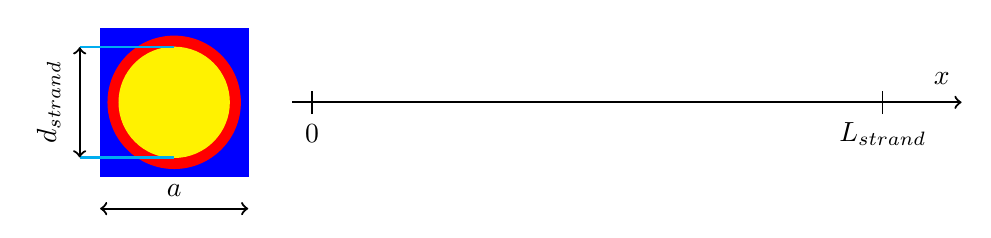
\begin{tikzpicture}[scale = 1]
        \filldraw[blue] (-0.941,-0.941) rectangle (0.941,0.941);
        \filldraw[red] (0,0) circle (0.7+0.07*2);
        \filldraw[yellow] (0,0) circle (0.7);
        \draw[thick, cyan] (-0.8*1.5,0.7) -- (0,0.7);
        \draw[thick, cyan] (-0.8*1.5,-0.7) -- (0,-0.7);
        \draw[black, thick, <->] (-0.75*1.6,0.7) -- (-0.75*1.6,-0.7);
        \node[scale = 1, rotate=90] at (-1.1*1.45, 0) {$d_\text{strand}$};
        \draw[thick,<->] (-0.941,-0.9*1.5) -- (0.941,-0.9*1.5);
        \node[scale = 1] at (0, -0.7*1.6) {$a$};
        \draw[thick,->] (1.5,0) -- (10.0,0);
        \draw[thin] (1.75,-0.15) -- (1.75,0.15);
        \draw[thin] (9,-0.15) -- (9,0.15);
        
        \node[scale = 1] at (9.75, 0.3) {$x$};
        \node[scale = 1] at (9, -0.4) {$L_\text{strand}$};
        \node[scale = 1] at (1.75, -0.4) {0};
        
    \end{tikzpicture}
    \caption{1D strand geometry.}
    \label{fig: 1d_strand_geometry}
\end{figure}

The parameters the skew quadrupole are presented in Table \ref{table:skew_quad_params_table}. None of the presented parameters does not change in any of further analyses presented in the thesis. Last two: $(i)$ residual resistivity ratio, RRR, $(ii)$ copper-to-superconductor ratio, $f_{Cu/Nb-Ti}$ come from a measured prototype of this magnet examined at INFN \cite{marco_prioli_mails}.

\begin{table}[h!]
    \caption{Geometrical parameters for skew quadrupole \cite{hl_lhc_tech_design_report_v01, marco_prioli_mails}.} 
    \vspace{-1.em} 
    \fontsize{10}{10}
    \selectfont 
    \renewcommand{\arraystretch}{1.5}
    \begin{center}
    \begin{tabular}{ ccc }  
    \hline
    Strand diameter, $d_\text{strand}$ & 0.7 & [mm] \\
    Strand side, $a$ & 0.941 & [mm] \\
    $f_{Cu/Nb-Ti}$ & 2.2 & [-] \\
    RRR & 193 & [-] \\  
    \hline 
    \end{tabular}
    \end{center}  
     \label{table:skew_quad_params_table} 
 \end{table}
